\documentclass{theozettel}

%%%%%%%%%%%%%%%%%%%%%%%%%%%%%%%%%%%%%%%%%%%%%%%%%%%%%%%%%%%%%%%%%%%%%%%%%%%%%%%%%%%%%%%%%%%%%%%%%%%%%%%%%%%%%%
% page geometry
%%%%%%%%%%%%%%%%%%%%%%%%%%%%%%%%%%%%%%%%%%%%%%%%%%%%%%%%%%%%%%%%%%%%%%%%%%%%%%%%%%%%%%%%%%%%%%%%%%%%%%%%%%%%%%
\geometry{
	left=20mm,
	right=20mm,
	top=25mm,
	bottom=20mm
}
%%%%%%%%%%%%%%%%%%%%%%%%%%%%%%%%%%%%%%%%%%%%%%%%%%%%%%%%%%%%%%%%%%%%%%%%%%%%%%%%%%%%%%%%%%%%%%%%%%%%%%%%%%%%%%

\pgfplotsset{compat=1.16}

\usepackage{dsfont}
\renewcommand{\phi}{\varphi}

\theoI{5}

\begin{document}
\punkteV{5.1}{5.2}{5.3}{5.4}{5.5}

\section*{Aufgabe 6.1} 




\section*{Aufgabe 6.2} 

\begin{center}
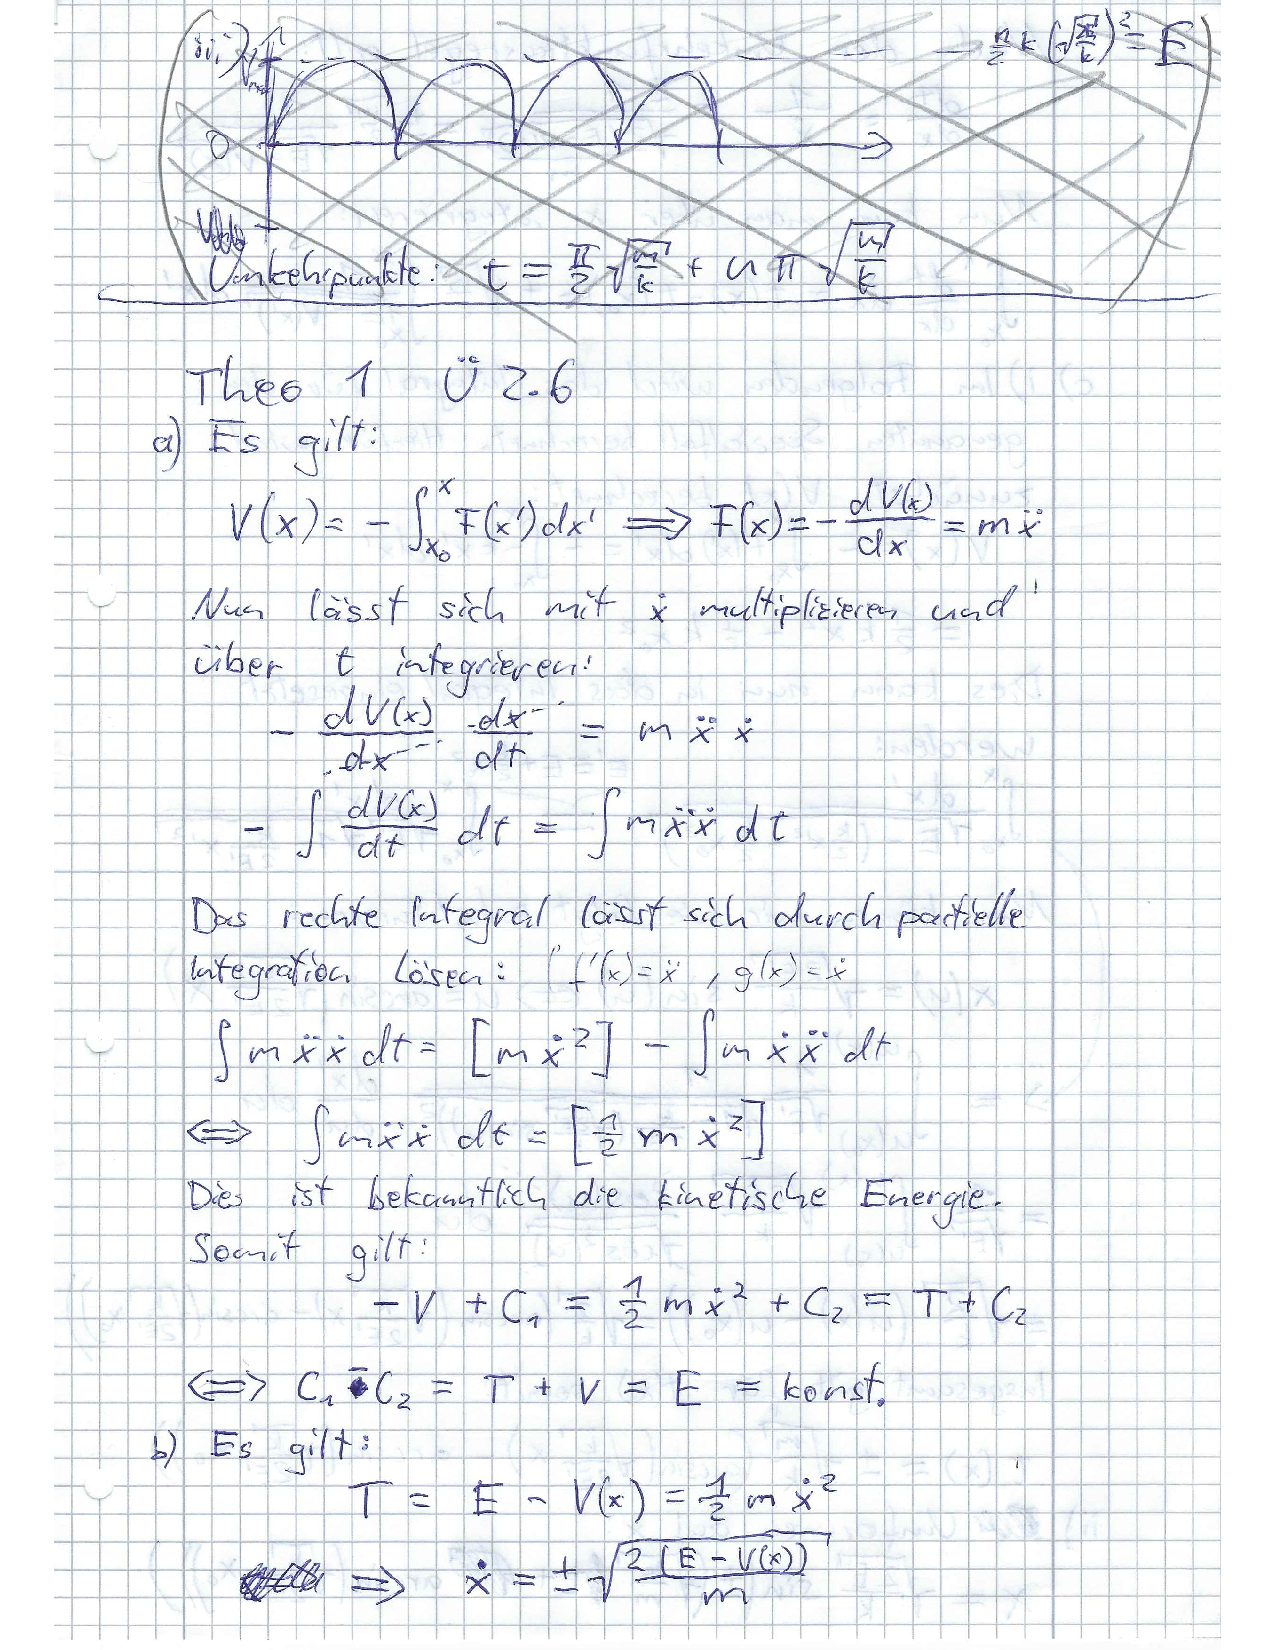
\includegraphics[width=15cm]{A2-Teil1.pdf}\\
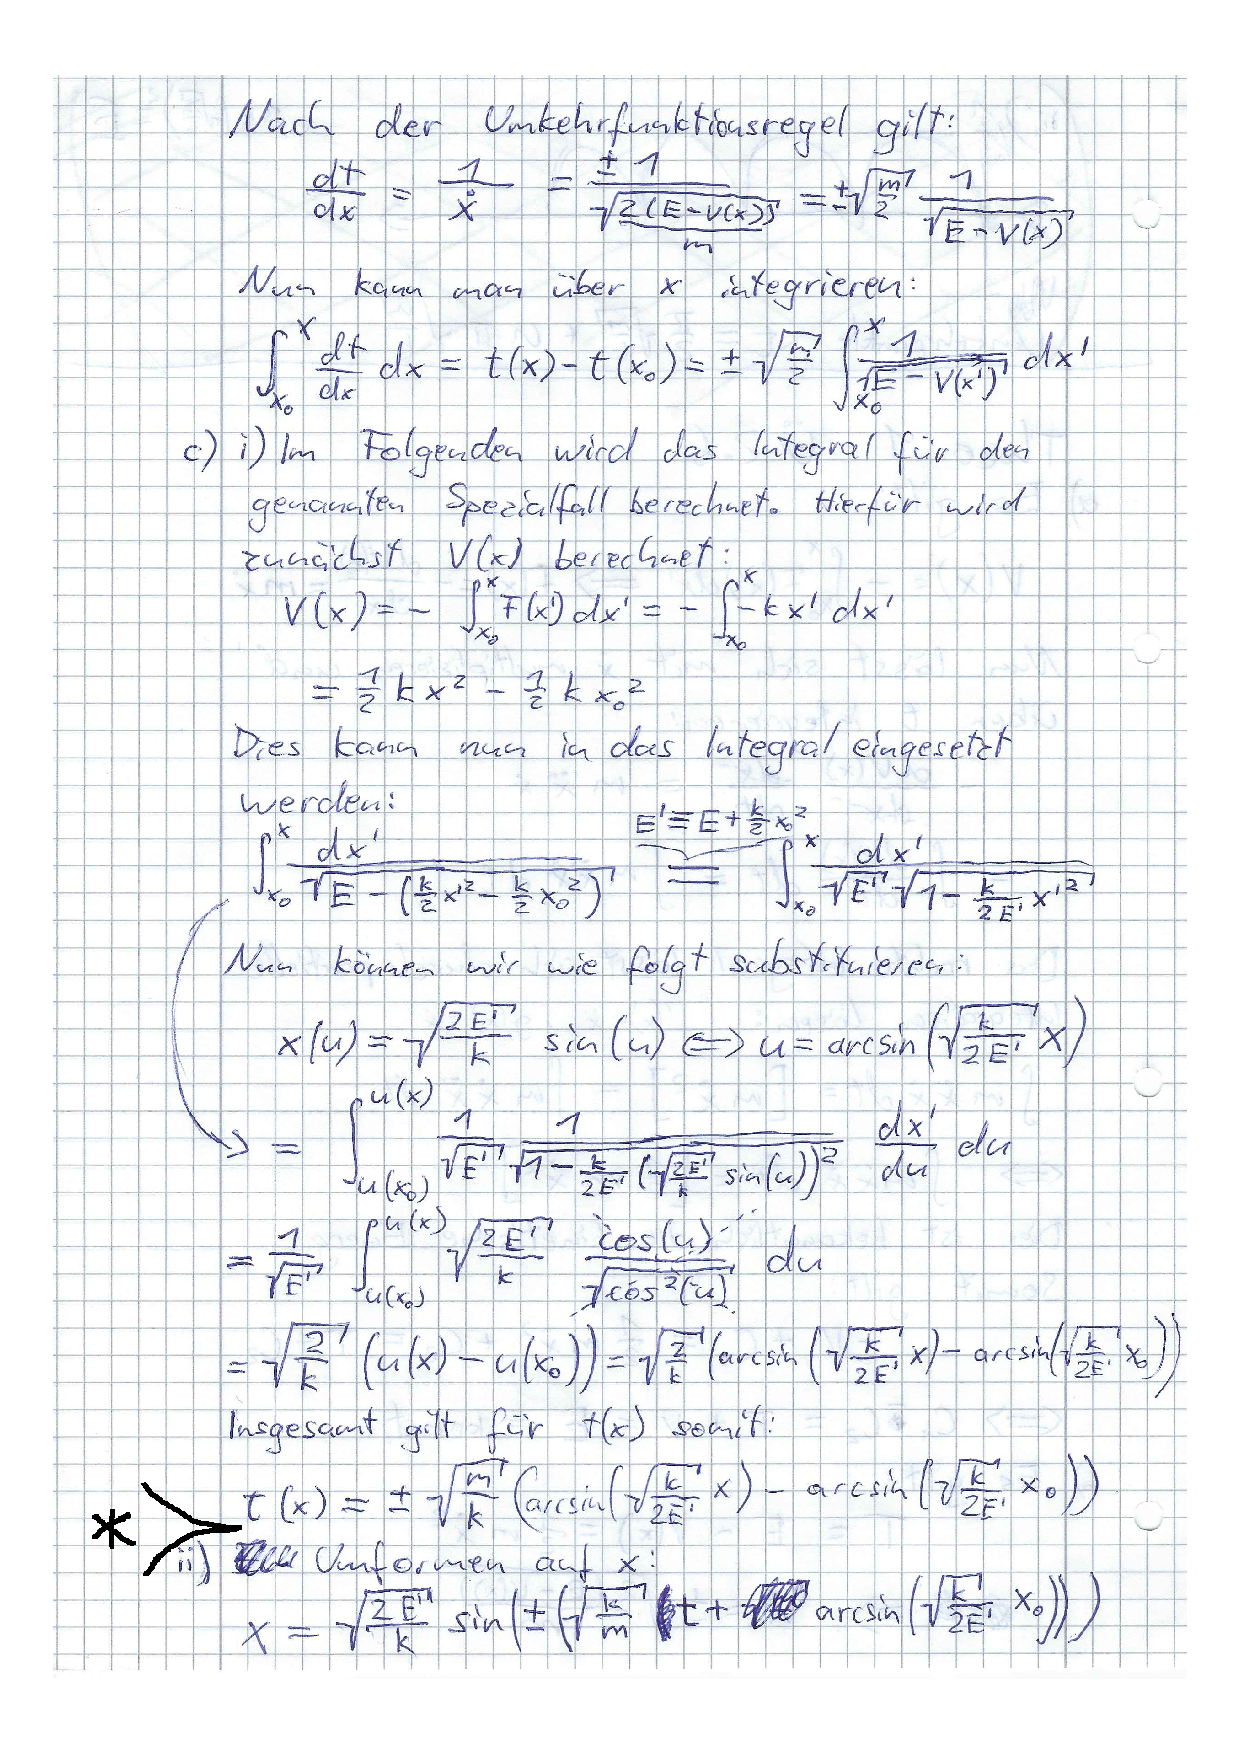
\includegraphics[width=15cm]{A2-Teil2_annotated.pdf}\\
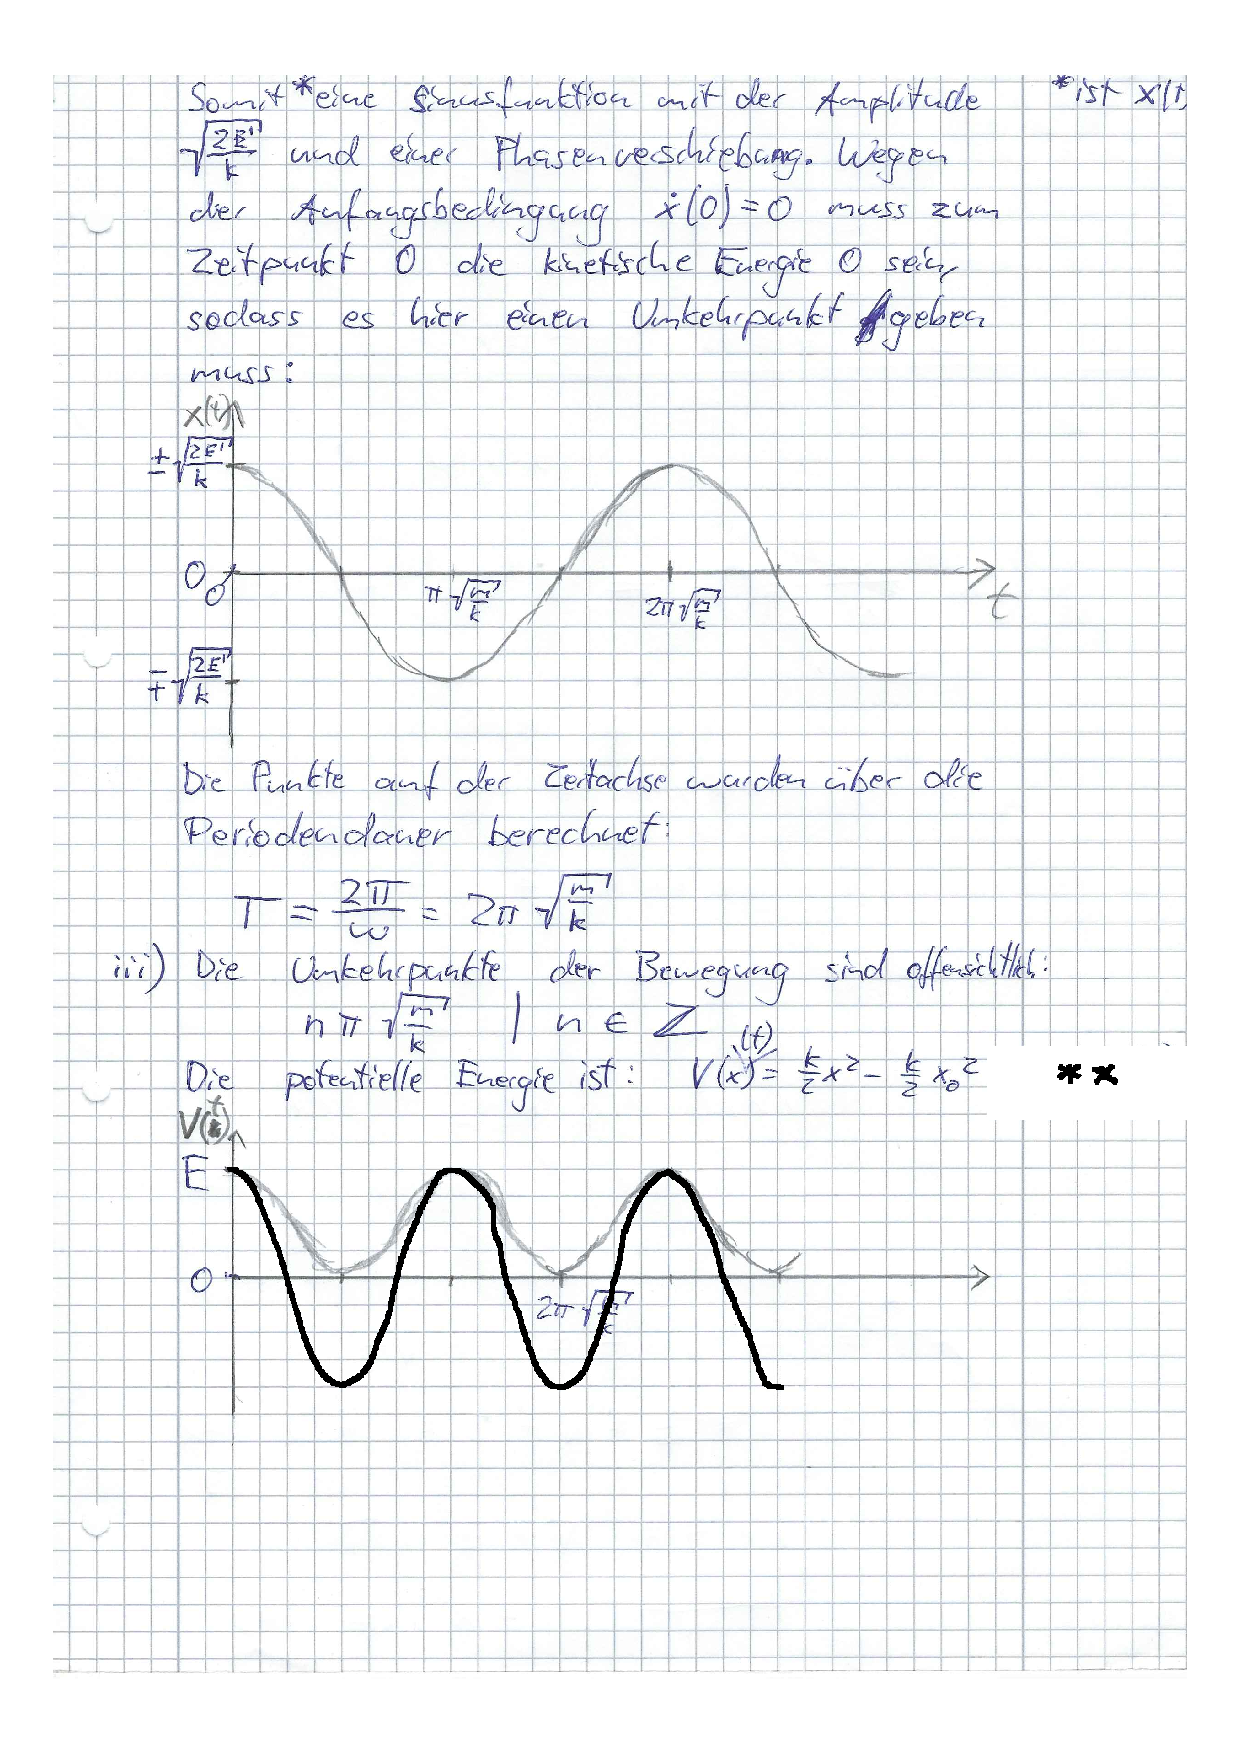
\includegraphics[width=15cm]{A2-Teil3_annotated.pdf}
\end{center}

* Ergänzung 1:

Wegen der Argumentation am Anfang vom 3. eingescannten Blatt gilt:

$$
\arcsin(\sqrt{\frac{k}{2 E'}} x_0) = \pm \frac{\pi}{2}
$$

Da gilt $\sin(x \pm \frac{\pi}{2}) = \pm \cos(x)$, lässt sich die Gleichung für $x$ vereinfachen zu (es wurde $E'$ resubstituiert):

$$
x(t) = \sqrt{\frac{2 E + k x_0^{2}}{k}} \cos(\sqrt{\frac{k}{m}} t)
$$

Dies ist auch in der ersten Skizze dargestellt.


** Ergänzung 2:

Bitte nur die schwarze, nicht die mit Bleistift gezeichnete Linie betrachten. Die Gleichung geht wie folgt weiter:

\begin{align}
\frac{k}{2}x^{2} - \frac{k}{2}x_0^{2} &= \frac{k}{2}\left(\sqrt{\frac{2 E + k x_0^{2}}{k}} \cos(\sqrt{\frac{k}{m}} t)\right)^{2} - \frac{k}{2}x_0^{2} \\
&= E \cos(\sqrt{\frac{k}{m}} t)^{2} + \frac{k}{2}x_0^{2} (\cos(\sqrt{\frac{k}{m}} t) - 1)^{2} \\
&= E \cos(\sqrt{\frac{k}{m}} t)^{2} - \frac{k}{2}x_0^{2} \sin(\sqrt{\frac{k}{m}} t)^{2}\\
&=  E \left( \cos(\sqrt{\frac{k}{m}} t)^{2} - \sin(\sqrt{\frac{k}{m}} t)^{2} \right)
\end{align}

Der letzte Umformungsschritt geht ebenfalls aus der Tatsache hervor, dass $\dot{x}(0) = 0$, sodass zum Zeitpunkt $0$ die gesamte Energie in der potentiellen Energie stecken muss.



\section*{Aufgabe 6.3} 





\section*{Aufgabe 6.4} 
Berechnen Sie
\subsection*{a)}die allgemeine Lösung der Differentialgleichung
\begin{align*}
y'=-\frac{2}{x}y+\frac{\ln x}{x^2}\tag*{(1)}\\
\end{align*}
Wir lösen zuerst den homogenen Teil:
\begin{align*}
\frac{\text{d}y}{\text{d}x}&=-\frac{2}{x}y\\
\text{Sep. der Var.:}\\
\frac{\text{d}y}{y}&=-\frac{2}{x}\text{d}x&&|\int\\
\int\frac{\text{d}y}{y}&=\int-\frac{2}{x}\text{d}x\\
\ln\left(y\right)&=-2\left(\ln\left(x\right)+\underline{c}\right)\\
\ln\left(y\right)&=-2\ln\left(x\right)-2\underline{c}&&|\text{$\ln$ auflösen}\\
y&=e^{-2\ln\left(x\right)}\cdot e^{-2\underline{c}}&&|c:=e^{-2\underline{c}}\\
y&=cx^{-2}\tag*{(2)}\\\\
\text{Variation der Kons.:} \ c&\rightarrow c\left(x\right)\\
y'&=-2\frac{c\left(x\right)}{x^2}+c'\left(x\right)x^{-2}\tag*{(3)}\\
\text{Setze (2) und (3) in (1) ein:}\\
-2\frac{c\left(x\right)}{x^3}+\frac{c'\left(x\right)}{x^2}&=-\frac{2}{x}\cdot\frac{c\left(x\right)}{x^2}+\frac{\ln\left(x\right)}{x^2}\\
\Leftrightarrow \frac{c'\left(x\right)}{x^2}&=\frac{\ln\left(x\right)}{x^2}\\
\Leftrightarrow c'\left(x\right)&=\ln\left(x\right)\\
\Rightarrow c\left(x\right)&=\int\text{d}x \ c'\left(x\right) =\int\text{d}x \ \ln\left(x\right)=x\ln\left(x\right)-x+\hat{c} \tag*{(4)}\\\\
\text{(4) in (2):}\\
y&=\left(x\ln\left(x\right)-x+\hat{c}\right)\cdot \frac{1}{x^2}\\
y&=\frac{\ln\left(x\right)-1}{x}-\frac{\hat{c}}{x^2}
\end{align*}
\newpage
\subsection*{b)} die Lösung des Anfangswertproblems
\begin{align*}
y'=-2xy+2xe^{-x^2} \tag*{(1)}, \ y\left(0\right)=2
\end{align*}
Wir bestimmen den homogenen Teil:
\begin{align*}
\frac{\text{d}y}{\text{d}x}&=-2xy\\
\text{Sep. der Var.:}\\
\frac{\text{d}y}{y}=-2x\text{d}x&&|\int\\
\int\text{d}y \ \frac{1}{y}&=-2\int\text{d}x \ x\\
\ln\left(y\right)&=-x^2-\hat{c}&&|\text{$\ln$ beseitigen}\\
y&=e^{-x^2-\hat{c}}\\
y&=e^{-x^2}\cdot e^{-\hat{c}}&&|c:=e^{-\hat{c}}\\
y&=ce^{-x^2}\tag*{(2)}\\\\
\text{Variation der Kons.:} \ c\rightarrow c\left(x\right)\\
y'&=c'\left(x\right)e^{-x^2}-2xe^{-x^2}c\left(x\right)\tag*{(3)}\\\\
\text{(2) und (3) in (1):}\\
c'\left(x\right)e^{-x^2}-2xe^{-x^2}&=-2xc\left(x\right)e^{-x^2}+2xe^{-x^2}\\
c'\left(x\right)e^{-x^2}&=2xe^{-x^2}\\
c'\left(x\right)&=2x\\
\Rightarrow c\left(x\right)&=\int\text{d}x \ c'\left(x\right)=\int\text{d}x \ 2x=x^2+\hat{c}\tag*{(4)}\\\\
\text{(4) in (1) ergibt allg. Lösung für Dgl.:}\\
y&=\left(x^2+\hat{c}\right)e^{-x^2}\\\\
\text{Anfangsbed.} \ y\left(0\right)=2 \ \text{einsetzen:}\\
y\left(0\right)&=\hat{c}=2\\
\Rightarrow y&=\left(x^2+2\right)e^{-x^2}
\end{align*}



\end{document}
